\section{Change of Variables in Multiple Integrals}\label{sec:jacobian}

% this was originally Schoolcraft

Given the difficulty of evaluating multiple integrals, the reader may be wondering if it is possible to simplify those integrals using a suitable substitution for the variables. The answer is yes, though it is a bit more complicated than the substitution method which you learned in single-variable calculus.\index{change of variable}

Recall that if you are given, for example, the definite integral
\[\int_1^2 x^3 \sqrt{x^2 - 1}\,dx ,\]
then you would make the substitution
\begin{align*}
u &= x^2 - 1 \Rightarrow x^2 = u + 1\\
du &= 2x\,dx\\
\intertext{which changes the limits of integration}
x &= 1 \Rightarrow u = 0\\
x &= 2 \Rightarrow u = 3
\end{align*}
so that we get
\begin{align*}
 \int_1^2 x^3 \sqrt{x^2 - 1}\,dx &= \int_1^2 \frac12 x^2 \cdot 2x \sqrt{x^2 - 1}\,dx\\
 &= \int_0^3 \frac12 (u+1)\sqrt{u}\,du\\
 &= \frac12 \int_0^3 \left( u^{3/2} + u^{1/2} \right)\,du \\
 &= \frac{14\sqrt3}5 .
\end{align*}
Let us take a different look at what happened when we did that substitution, which will give some motivation for how substitution works in multiple integrals. First, we let $u = x^2 - 1$. On the interval of integration $[ 1,2 ]$, the function $x \mapsto x^2 - 1$ is strictly increasing (and maps $[ 1,2 ]$ onto $[ 0,3 ]$) and hence has an inverse function (defined on the interval $[ 0,3 ]$). That is, on $[ 0,3 ]$ we can define $x$ as a function of $u$, namely
\[x = g(u) = \sqrt{u+1} .\]
Then substituting that expression for $x$ into the function $f(x) = x^3 \sqrt{x^2 - 1}$ gives
\[f(x) = f(g(u)) = (u+1)^{3/2} \sqrt{u} ,\]
and we see that
\begin{align*}
 \frac{dx}{du} = g\primeskip'(u) \Rightarrow dx &= g\primeskip'(u)\,du\\
 dx &= \frac12 (u+1)^{-1/2}\,du ,
\end{align*}
so since
\begin{align*}
 g(0) = 1 \Rightarrow 0 = g^{-1} (1)\\
 g(3) = 2 \Rightarrow 3 = g^{-1} (2)\\
\end{align*}
then performing the substitution as we did earlier gives
\begin{align*}
 \int_1^2 f(x)\,dx &= \int_1^2 x^3 \sqrt{x^2 - 1}\,dx\\
 &= \int_0^3 \frac12(u+1)\sqrt{u}\,du ,\text{ which can be written as}\\
 &= \int_0^3 (u+1)^{3/2} \sqrt{u} \, \cdot \frac12 (u+1)^{-1/2}\,du ,\text{ which means}\\
 \int_1^2 f(x)\,dx &= \int_{g^{-1}(1)}^{g^{-1}(2)} f(g(u))\,g\primeskip'(u)\,du .
\end{align*}

In general, if $x = g(u)$ is a one-to-one, differentiable function from an interval $[ c,d ]$ (which you can think of as being on the ``$u$-axis'') onto an interval $[ a,b ]$ (on the $x$-axis), which means that $g\primeskip'(u) \ne 0$ on the interval $(c,d)$, so that $a=g(c)$ and $b=g(d)$, then $c=g^{-1}(a)$ and $d=g^{-1}(b)$, and
\[\int_a^b f(x)\,dx = \int_{g^{-1}(a)}^{g^{-1}(b)} f(g(u))\,g\primeskip'(u)\,du .\]
This is called the \emph{change of variable} formula for integrals of single-variable functions, and it is what you were implicitly using when doing integration by substitution. This formula turns out to be a special case of a more general formula which can be used to evaluate multiple integrals. We will state the formulas for double and triple integrals involving real-valued functions of two and three variables, respectively. We will assume that all the functions involved are continuously differentiable and that the regions and solids involved all have ``reasonable'' boundaries. The proof of the following theorem is beyond the scope of the text.% See \cite[\S\,15.32 and \S\,15.62]{tm} for all the details.

\theorem{thm:changevarint}{Change of Variables Formula for Multiple Integrals}{Let $x=x(u,v)$ and $y=y(u,v)$ define a one-to-one mapping of a region $R'$ in the $uv$-plane onto a region $R$ in the $xy$-plane such that the determinant\index{change of variable}
  \begin{equation}\label{eqn:jacob2}
   J(u,v) =
    \begin{vmatrix}
     \dfrac{\partial x}{\partial u} & \dfrac{\partial x}{\partial v}\vspace{2mm}\\
     \dfrac{\partial y}{\partial u} & \dfrac{\partial y}{\partial v}
    \end{vmatrix}
  \end{equation}
  is never $0$ in $R'$. Then
  \begin{equation}\label{eqn:changevarint2}
   \iint_{R} f(x,y)\,dA(x,y)
   = \iint_{R'} f(x(u,v),y(u,v))\,\abs{J(u,v)}\,dA(u,v) .
  \end{equation}
  We use the notation $dA(x,y)$ and $dA(u,v)$ to denote the area element in the $(x,y)$ and $(u,v)$ coordinates, respectively.
  
  Similarly, if $x=x(u,v,w)$, $y=y(u,v,w)$ and $z=z(u,v,w)$ define a one-to-one mapping of a solid $S'$ in $uvw$-space onto a solid $S$ in $xyz$-space such that the determinant
  \begin{equation}\label{eqn:jacob3}
   J(u,v,w) =
    \begin{vmatrix}
     \dfrac{\partial x}{\partial u} & \dfrac{\partial x}{\partial v} & \dfrac{\partial x}{\partial w}\vspace{2mm}\\
     \dfrac{\partial y}{\partial u} & \dfrac{\partial y}{\partial v} & \dfrac{\partial y}{\partial w}\vspace{2mm}\\
     \dfrac{\partial z}{\partial u} & \dfrac{\partial z}{\partial v} & \dfrac{\partial z}{\partial w}
    \end{vmatrix}
  \end{equation}
  is never $0$ in $S'$, then
  \begin{multline}\label{eqn:changevarint3}
   \iiint_{S} f(x,y,z)\,dV(x,y,z) =\\
   \iiint_{S'} f(x(u,v,w),y(u,v,w),z(u,v,w))\,\abs{J(u,v,w)}\,dV(u,v,w).
  \end{multline}}

The determinant $J(u,v)$ in \autoeqref{eqn:jacob2} is called the \textbf{Jacobian} of $x$ and $y$ with respect to $u$ and $v$, and is sometimes written as\index{Jacobian}
\[J(u,v) = \frac{\partial (x,y)}{\partial (u,v)} .\]
Similarly, the Jacobian $J(u,v,w)$ of three variables is sometimes written as
\[J(u,v,w) = \frac{\partial (x,y,z)}{\partial (u,v,w)} .\]
Notice that \autoeqref{eqn:changevarint2} is saying that $dA(x,y) = \abs{J(u,v)}\,dA(u,v)$, which you can think of as a two-variable version of the relation $dx = g\primeskip'(u)\,du$ in the single-variable case.

\youtubeVideo{Bw5yEqwMjQU}{Jacobian}

The following example shows how the change of variables formula is used.\index{$\dfrac{\partial (x,y,z)}{\partial (u,v,w)}$}

\example{ex_simple_Jacobian}{Change of Variables}{Evaluate $\ds\iint_{R} e^{\frac{x-y}{x+y}} \,dA$, where $R= \lbrace (x,y): x \ge 0, y \ge 0,
 x + y \le 1 \rbrace$.}{First, note that evaluating this double integral \emph{without} using substitution is probably impossible, at least in a closed form. By looking at the numerator and denominator of the exponent of $e$, we will try the substitution $u=x-y$ and $v=x+y$. To use the change of variables \autoeqref{eqn:changevarint2}, we need to write both $x$ and $y$ in terms of $u$ and $v$. So solving for $x$ and $y$ gives $x=\frac12(u+v)$ and $y=\frac12(v-u)$. In \autoref{fig:exyint} below, we see how the mapping $x=x(u,v)=\frac12(u+v)$,
 $y=y(u,v)=\frac12(v-u)$ maps the region $R'$ onto $R$ in a one-to-one manner.
 
\begin{lxfigure}
 \centering
  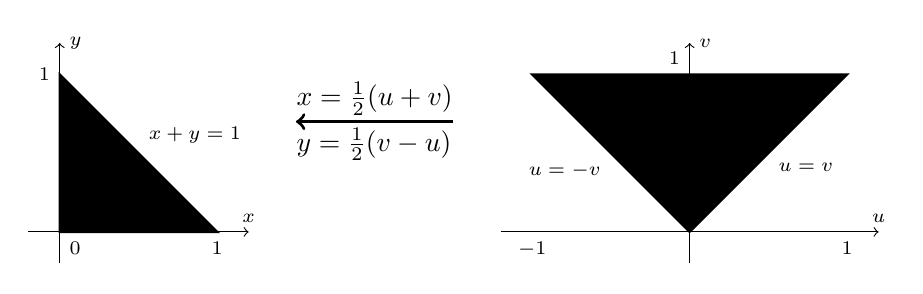
\begin{tikzpicture}[scale=2]
   % the left area
   \draw[draw={\colorone},fill={\coloronefill},thick]
    (0,0)--(1,0)--node[pos=.5,above right]{\scriptsize$x+y=1$}(0,1)--cycle;
   \draw[draw={\colorone},->](-.2,0)
    --node[above,color=black,pos=1]{\scriptsize$x$}(1.2,0);
   \node[below]at(1,0){\scriptsize$1$};
   \draw[draw={\colorone},->](0,-.2)
    --node[right,color=black,pos=1]{\scriptsize$y$}(0,1.2);
   \node[left]at(0,1){\scriptsize$1$};
   \node[below right] at (0,0) {\scriptsize$0$};
   \node at (0.2,0.2) {\small $R$};
   % the arrow
   \draw[->,very thick](2.5,.7)
    --node[pos=.5]{\begin{tabular}{l}$x=\frac12(u+v)$\\[1ex]$y=\frac12(v-u)$\end{tabular}}(1.5,.7);
   % the right area
   \draw[draw={\colorone},fill={\coloronefill},thick](4,0)
    --node[pos=.5,below right,color=black]{\scriptsize$u=v$}(5,1)--(3,1)
    --node[pos=.5,below left ,color=black]{\scriptsize$u=-v$}(4,0);
   \draw[draw={\colorone},->](2.8,0)
    --node[above,color=black,pos=1]{\scriptsize$u$}(5.2,0);
   \node[below]at(3,0){\scriptsize$-1$};
   \node[below]at(5,0){\scriptsize$1$};
   \draw[draw={\colorone},->](4,-.2)
    --node[right,color=black,pos=1]{\scriptsize$v$}(4,1.2);
   \node[above left]at(4,1){\scriptsize$1$};
   \node[right]at(4,.6){$R'$};
  \end{tikzpicture}
 \caption{The regions $R$ and $R'$}
 \label{fig:exyint}
\end{lxfigure}

 Now we see that
 \[
 J(u,v) =
   \begin{vmatrix}
    \dfrac{\partial x}{\partial u} & \dfrac{\partial x}{\partial v}\vspace{2mm}\\
    \dfrac{\partial y}{\partial u} & \dfrac{\partial y}{\partial v}
   \end{vmatrix}
   =\begin{vmatrix}
    \frac12 & \frac12\vspace{2mm}\\
    -\frac12 & \frac12
   \end{vmatrix}
   = \frac12 \Rightarrow \abs{J(u,v)} = \abs{\frac12} = \frac12 ,
 \]
 so using horizontal slices in $R'$, we have
 \begin{align*}
  \iint_{R} e^{\frac{x-y}{x+y}} \,dA &= \iint_{R'} f(x(u,v),y(u,v))\,\abs{J(u,v)}\,dA\\
  &= \int_0^1 \int_{-v}^v e^{\frac uv} \, \frac12\,du\,dv\\
  &= \int_0^1 \left(\left. \frac v2 e^{\frac uv} \,\right|_{u=-v}^{u=v} \right) \,dv\\
  &= \int_0^1 \frac v2 (e - e^{-1})\,dv\\
  &= \left.\frac{v^2}4 (e - e^{-1}) \,\right|_{0}^{1}
  = \frac14 \left( e - \frac1e \right) = \frac{e^2 - 1}{4e}.\eoehere
 \end{align*}}

The change of variables formula can be used to evaluate double integrals in polar coordinates. Letting
\[
 x = x(r,\theta) = r\cos \theta \quad \text{and} \quad y = y(r,\theta) = r\sin \theta ,
\]
we have
\[
 J(u,v) =
  \begin{vmatrix}
   \dfrac{\partial x}{\partial r} & \dfrac{\partial x}{\partial \theta}\vspace{2mm}\\
   \dfrac{\partial y}{\partial r} & \dfrac{\partial y}{\partial \theta}
  \end{vmatrix} =
  \begin{vmatrix}
   \cos \theta & -r\sin \theta\vspace{2mm}\\
   \sin \theta & r\cos \theta
  \end{vmatrix}= r\cos^2 \theta + r\sin^2 \theta = r
  \Rightarrow \abs{J(u,v)} = \abs{r} = r ,
\]
which verifies \autoref{idea:doublepol}.
%so we have the following formula:

%\keyidea{idea_polar_int}{Double Integral in Polar Coordinates}{
% \begin{equation}\label{eqn:polarint}
%  \iint_{R} f(x,y)\,dx\,dy
%  = \iint_{R'} f(r\cos \theta,r\sin \theta)\,r\,dr\,d\theta ,
% \end{equation}\index{double integral!polar coordinates}\index{coordinates!polar}
% where the mapping $x=r\cos \theta$, $y=r\sin \theta$ maps the region $R'$ in the $r\theta$-plane onto the region $R$ in the $xy$-plane in a one-to-one manner.}

%\example{ex_polar_parab}{Integrating in Polar Coordinates}{Find the volume $V$ inside the paraboloid $z=x^2 + y^2$ for $0 \le z \le 1$.}{Using vertical slices, we see that
%\[V = \iint_{R} (1 - z)\,dA = \iint_{R} (1 - (x^2 + y^2 ))\,dA ,\]
%where $R = \lbrace (x,y): x^2 + y^2 \le 1 \rbrace$ is the unit disk in $\mathbb{R}^2$ (see \autoref{fig_parab}). In polar coordinates $(r,\theta)$ we know that $x^2 + y^2 = r^2$ and that the unit disk $R$ is the set $R' = \lbrace (r,\theta):0 \le r \le 1, 0 \le \theta \le 2\pi \rbrace$. Thus,
%\mtable{$z=x^2 + y^2$ for \autoref{ex_polar_parab}}{fig_parab}{\begin{tikzpicture}
%  \usetikzlibrary{arrows}
%  \definecolor{insideo}{HTML}{798084}
%  \definecolor{insidei}{HTML}{F0F0F0}
%  \definecolor{outer}{HTML}{424296}
%  \definecolor{inner}{HTML}{D8D8FF}
%  \shadedraw [left color=insideo,right color=insideo,middle color=insidei] (0,3) ellipse (2 and 0.7);
%  \shadedraw [left color=outer,right color=outer,middle color=inner]
%  (2,3) arc (360:180:2 and 0.7) -- (-2,3) parabola bend (0,0) (2,3);
%  \draw [dashed,line width=0.2pt] (-2,3) -- (2,3);
%  \draw [dashed,line width=0.2pt] (-0.66,2.34) -- (0.66,3.66);
%  \draw [line width=0.2pt] (-0.66,2.34) parabola [bend at end] (0,0);
%  \draw [dashed,line width=0.2pt] (0.66,3.66) parabola [bend at end] (0,0);
%  \draw [line width=0.2pt] (-1.25,1.2) arc (180:360:1.25 and 0.4);
%  \draw [dashed,line width=0.2pt] (-1.25,1.2) arc (180:0:1.25 and 0.4);
%  \draw [black!60,line width=0.3pt,-latex] (-2,0) -- (2,0,0);
%  \draw [black!60,line width=0.3pt,-latex] (0,0) -- (0,4,0);
%  \draw [black!60,line width=0.3pt,-latex] (0,0) -- (0,0,2);
%  \node[above]at(2,0){\small$y$};
%  \node[right]at(0,4){\small$z$};
%  \node[right]at(0,0,2){\small$x$};
%  \node[below right]at(0,0){\small$0$};
%%  \pgfputat{\pgfpointxyz{1.9}{0.2}{0}}{\pgfbox[center,center]{\small $y$}};
%%  \pgfputat{\pgfpointxyz{0.2}{3.9}{0}}{\pgfbox[center,center]{\small $z$}};
%%  \pgfputat{\pgfpointxyz{0.2}{0}{1.8}}{\pgfbox[center,center]{\small $x$}};
%%  \pgfputat{\pgfpointxyz{0.05}{-0.2}{0}}{\pgfbox[center,center]{\small $0$}};
%  \node [right] at (1.5,3.7) {\small $x^2 + y^2 = 1$};
%  \node [above left] at (0,3) {\small $1$};
% \end{tikzpicture}}%
% \begin{align*}
%  V &= \int_0^{2\pi} \int_0^1 (1 - r^2 )\,r\,dr\,d\theta\\
%   &= \int_0^{2\pi} \int_0^1 (r - r^3 )\,dr\,d\theta\\
%   &= \int_0^{2\pi} \left( \left.\frac{r^2}2 - \frac{r^4}4 \,\right|_{r=0}^{r=1} \right) \,d\theta\\
%   &= \int_0^{2\pi} \frac14 \,d\theta\\
%   &= \frac\pi2.\eoehere
% \end{align*}}

%\example{ex_polar_cone}{Integrating in Polar Coordinates}{Find the volume $V$ inside the cone $z=\sqrt{x^2 + y^2}$ for $0 \le z \le 1$.}{%
% \mtable{$z=\sqrt{x^2 + y^2}$ for \autoref{ex_polar_cone}}{fig_cone}{\begin{tikzpicture}
%  \usetikzlibrary{arrows}
%  \definecolor{insideo}{HTML}{798084}
%  \definecolor{insidei}{HTML}{F0F0F0}
%  \definecolor{outer}{HTML}{424296}
%  \definecolor{inner}{HTML}{D8D8FF}
%  \shadedraw [left color=insideo,right color=insideo,middle color=insidei] (1.3,2) arc (0:180:1.3 and .5) --
%   (-1.3,2) arc (180:360:1.3 and .5);
%  \shadedraw [left color=outer,right color=outer,middle color=inner] (0,0) -- (-1.3,2) arc (180:360:1.3 and .5)
%   -- (0,0);
%  \draw [dashed,line width=0.2pt] (-1.3,2) -- (1.3,2);
%  \draw [black!60,line width=0.3pt,-latex] (-2,0) -- (2,0,0);
%  \draw [black!60,line width=0.3pt,-latex] (1,1) -- (0,0,2);
%  \draw [black!60,line width=0.3pt,-latex] (0,-0.5) -- (0,2.9,0);
%  \node[above]at(2,0){\small$y$};
%  \node[right]at(0,3){\small$z$};
%  \node[right]at(0,0,2){\small$x$};
%  \node[below right]at(0,0){\small$0$};
%%  \pgfputat{\pgfpointxyz{1.9}{0.2}{0}}{\pgfbox[center,center]{\small $y$}};
%%  \pgfputat{\pgfpointxyz{0.2}{2.8}{0}}{\pgfbox[center,center]{\small $z$}};
%%  \pgfputat{\pgfpointxyz{0.2}{0}{1.8}}{\pgfbox[center,center]{\small $x$}};
%%  \pgfputat{\pgfpointxyz{0.15}{-0.2}{0}}{\pgfbox[center,center]{\small $0$}};
%  \node [above] at (1.3,2.4) {\small $x^2 + y^2 = 1$};
%  \node [above left] at (0,2) {\small $1$};
% \end{tikzpicture}
% }
% Using vertical slices, we see that
% \[
%  V = \iint_{R} (1 - z)\,dA
%  = \iint_{R} \left( 1 - \sqrt{x^2 + y^2} \right) \,dA ,
% \]
% where $R = \lbrace (x,y): x^2 + y^2 \le 1 \rbrace$ is the unit disk in $\mathbb{R}^2$ (see \autoref{fig_cone}). In polar coordinates $(r,\theta)$ we know\\that $\sqrt{x^2 + y^2} = r$ and that the unit disk $R$ is the set\\$R' = \lbrace (r,\theta):0 \le r \le 1, 0 \le \theta \le 2\pi \rbrace$. Thus,
% \begin{align*}
%  V &= \int_0^{2\pi} \int_0^1 (1 - r)\,r\,dr\,d\theta\\
%   &= \int_0^{2\pi} \int_0^1 (r - r^2 )\,dr\,d\theta\\
%   &= \int_0^{2\pi} \left( \left.\frac{r^2}2 - \frac{r^3}3 \,\right|_{r=0}^{r=1} \right) \,d\theta\\
%   &= \int_0^{2\pi} \frac16 \,d\theta\\
%   &= \frac\pi3.\eoehere
% \end{align*}}

In a similar fashion, it can be shown (see Exercises \ref{pr_cyl_jac} and \ref{pr_sph_jac}) that triple integrals in cylindrical and spherical coordinates take the following forms:

\keyidea{idea_cylin_int}{Triple Integral in Cylindrical Coordinates}{%
 \begin{equation}\label{eqn:cylinderint}
  \iiint_{S} f(x,y,z)\,dx\,dy\,dz = \iiint_{S'} f(r\cos \theta,r\sin \theta,z)\,r\,dr\,d\theta\,dz ,
 \end{equation}\index{triple integral!cylindrical coordinates}
 where the mapping $x=r\cos \theta$, $y=r\sin \theta$, $z=z$ maps the solid $S'$ in  $r\theta z$-space onto the solid $S$ in $xyz$-space in a one-to-one manner.}

\keyidea{idea_sphere_int}{Triple Integral in Spherical Coordinates}{\mbox{}\\[-2\baselineskip]
 \begin{multline}\label{eqn:sphereint}
  \iiint_S f(x,y,z)\,dx\,dy\,dz =\\
  \iiint_{S'} f(\rho\sin \phi\,\cos \theta,\rho\sin \phi\,\sin \theta,\rho\cos \phi)
  \,\rho^2 \,\sin \phi \,d\rho\,d\phi\,d\theta ,
 \end{multline}\index{triple integral!spherical coordinates}
 where the mapping $x=\rho\sin \phi\,\cos \theta$, $y=\rho\sin \phi\,\sin \theta$, $z=\rho\cos \phi$ maps the solid $S'$ in $\rho\phi\theta$-space onto the solid $S$ in $xyz$-space in a one-to-one manner.}
 
\example{exmp_volsphere}{Finding the Volume of a Sphere}{For $a > 0$, find the volume $V$ inside the sphere $S = x^2 + y^2 + z^2 = a^2$.}{We see that $S$ is the set $\rho = a$ in spherical coordinates, so
 \begin{align*}
  V &= \iiint_S 1\,dV
   = \int_0^{2\pi} \int_0^\pi \int_0^a 1 \,\rho^2 \,\sin \phi \,d\rho\,d\phi\,d\theta\\
   &= \int_0^{2\pi} \int_0^\pi \left( \left.\frac{\rho^3}3\,\right|_{\rho=0}^{\rho=a}\right)\,\sin \phi \,d\phi\,d\theta
   = \int_0^{2\pi} \int_0^{\pi} \frac{a^3}3\,\sin \phi\,d\phi\,d\theta\\
   &= \int_0^{2\pi} \left( \left. -\frac{a^3}3\,\cos \phi\,\right|_{\phi=0}^{\phi=\pi} \right) \,d\theta
   = \int_0^{2\pi} \frac{2a^3}3\,d\theta
   = \frac{4\pi a^3}3 .\eoehere
 \end{align*}}

This chapter investigated the natural follow--on to partial derivatives: iterated integration. We learned how to use the bounds of a double integral to describe a region in the plane using both rectangular and polar coordinates, then later expanded to use the bounds of a triple integral to describe a region in space. We used double integrals to find volumes under surfaces, surface area, and the center of mass of lamina; we used triple integrals as an alternate method of finding volumes of space regions and also to find the center of mass of a region in space.

Integration does not stop here. We could continue to iterate our integrals, next investigating ``quadruple integrals'' whose bounds describe a region in 4--dimensional space (which are very hard to visualize). We can also look back to ``regular'' integration where we found the area under a curve in the plane. A natural analogue to this is finding the ``area under a curve,'' where the curve is in space, not in a plane. These are just two of many avenues to explore under the heading of ``integration.''

\printexercises{exercises/13_Jacobian_exercises}
